\subsection{Introduction (Tuan Anh)}
	We obtained the data from the ECG database from the PhysioNet database located at \url{http://physionet.org/physiobank/database/apnea-ecg/}. The data consists of 35 labelled training records and 35 unlabelled records (used for the CinC Challenge 2000 competition). The recordings vary from less than 7 hours to 10 hours each and include continuous digitised ECG signal and, in the case of the training data, a set of apnoea annotations derived by human experts. The continuous signal is sampled at the rate of 100 Hz and the annotations are available at every 6000 samples (i.e. every minute) of the signal indicating the presence of apnoea at that time. One such record is shown in Figure \ref{fig:visualiseData}.

	\begin{figure}[ht!]
		\centering
			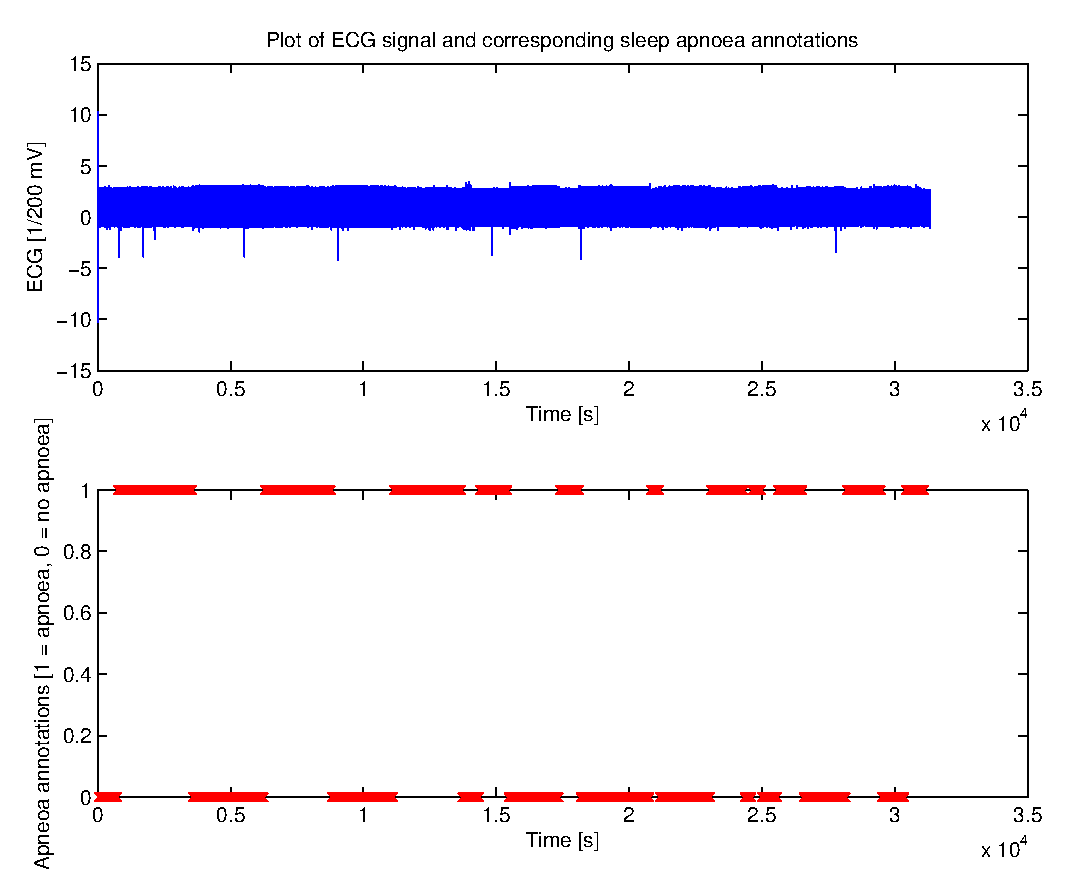
\includegraphics{drawings/visualiseData.eps}
		\caption{One training record}
		\label{fig:visualiseData}
	\end{figure}